\chapter{Organisation du projet}

Nous avons choisi de mettre en place un MVC (Model View Controller). On retrouve ainsi
un package View, un package Model et un package Controller. Le Controller contient
un objet ``MouseEvents'' présentant tous les évènements sours réalisables ainsi qu'une
classe ``Controller'' servant à lancer l'application et à instancier l'application.
Cette dernière lancera donc la View et instanciera un Model. Nous avons
fait le choix d'avoir un Model static disponible depuis la classe ``Main'', lançant
le programme et instanciant le Controller. Cela nous permettra d'y accèder aisément.
Une première version présentait le Model comme étant un singleton, partant du principe que ce dernier était unique. Cependant, cette idée fut abandonnée lors
de la mise en place du undo/redo à l'aide du design pattern Memento.
\\
Le Model se présente ainsi:

\hspace{2.3cm}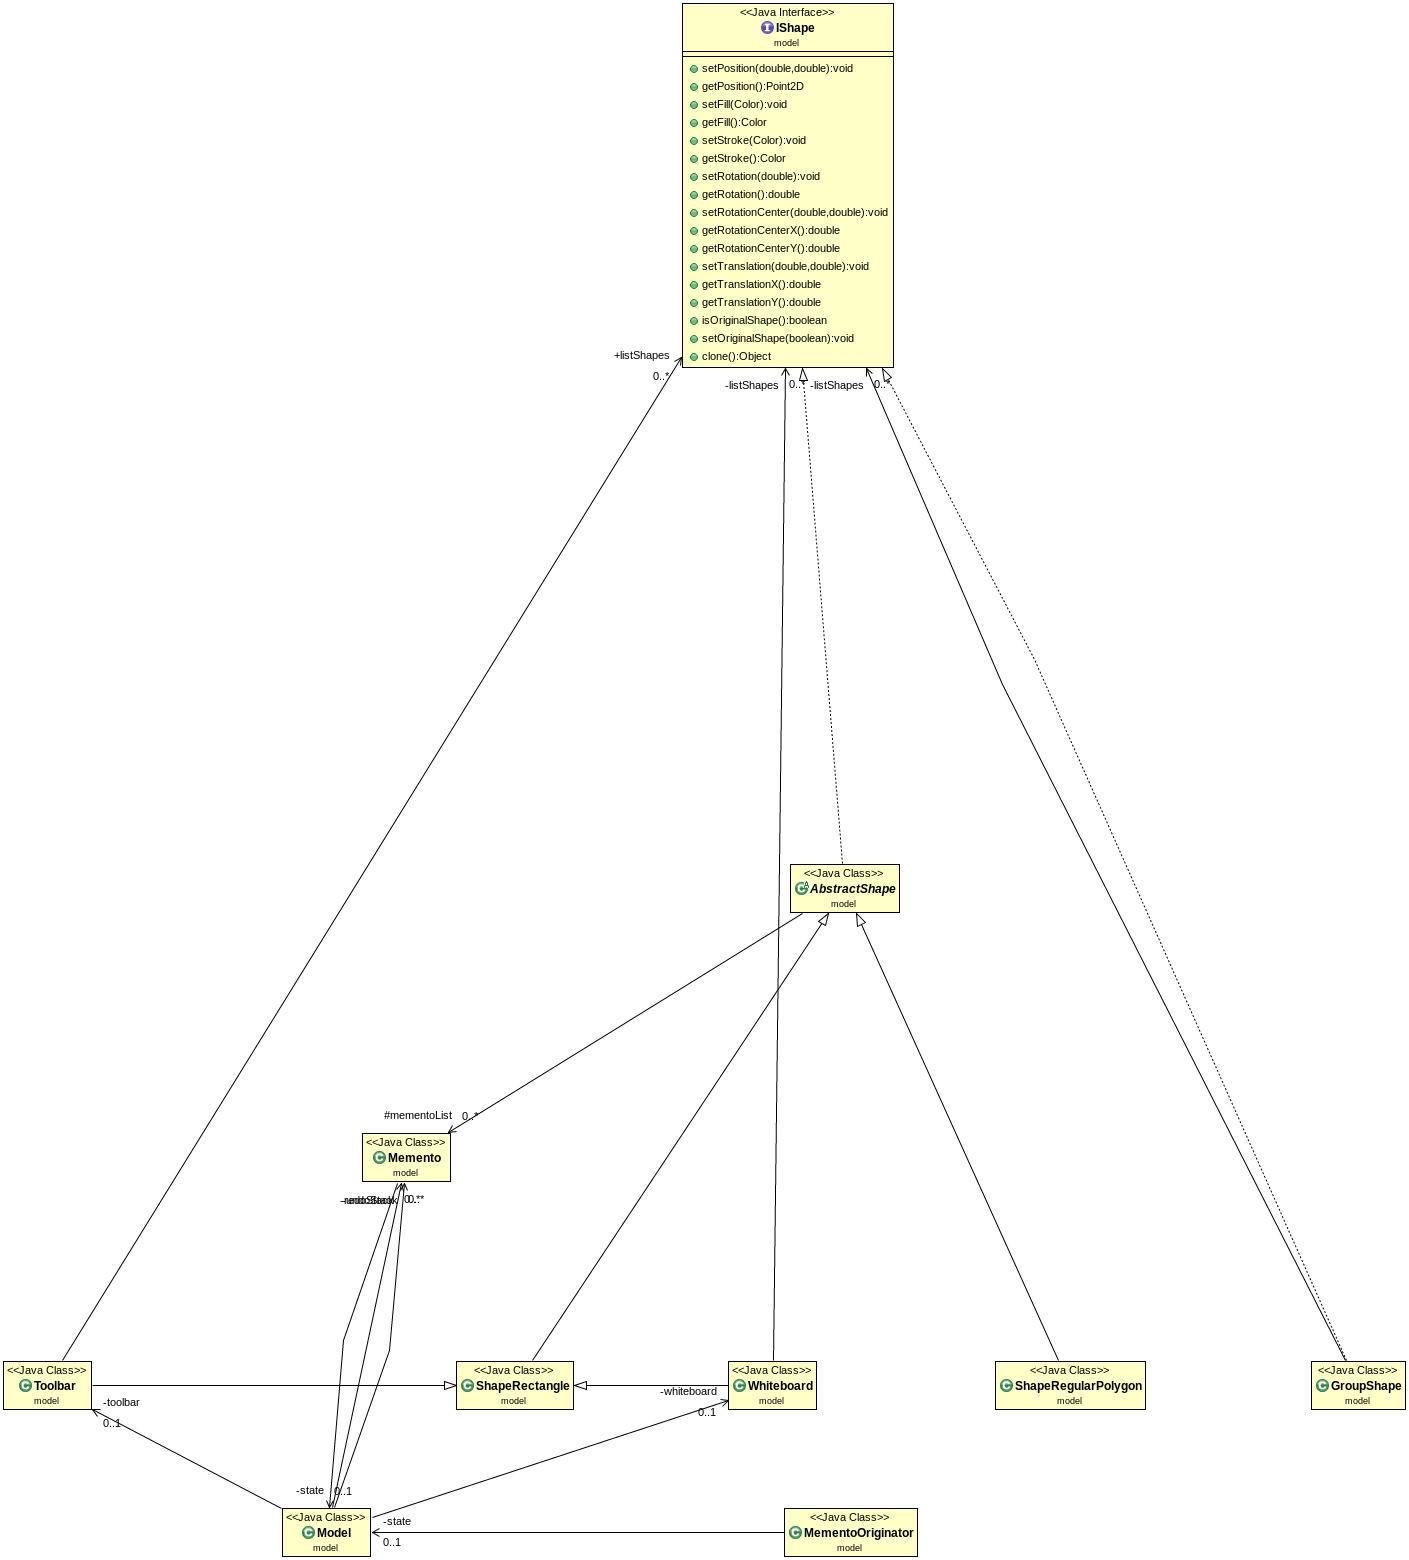
\includegraphics[scale=0.145]{../images/uml_model.png}
